\documentclass[tikz,border=10pt,12pt,x11names]{standalone}
\usepackage{tikz}
\usetikzlibrary{circuits.logic.US} % TiKZ Library for US Logic Circuits.
\begin{document}

	\begin{tikzpicture}[circuit logic US,
						tiny circuit symbols,
						every circuit symbol/.style={
						fill=white,draw}]

		\node[draw] at (-2.0bp,2.0bp) {module1};

		\node[draw] (a) at (27.0bp,18.0bp) {a};
		\node[draw] (b) at (27.0bp,72.0bp) {b};
		\node[draw] (c) at (27.0bp,126.0bp) {c};
		\node[draw] (d) at (27.0bp,180.0bp) {d};
		\node[draw] (cout) at (27.0bp,234.0bp) {cout};
		\node[draw] (e) at (27.0bp,288.0bp) {e};
		\node[draw] (f) at (27.0bp,342.0bp) {f};
		\node[draw] (g) at (27.0bp,396.0bp) {g};
		\node[draw] (h) at (27.0bp,450.0bp) {h};
		\node[draw] (cin) at (27.0bp,504.0bp) {cin};
		\node[draw] (r) at (27.0bp,558.0bp) {r};
		\node[draw] (s) at (27.0bp,612.0bp) {s};
		\node[draw] (t) at (27.0bp,666.0bp) {t};
		\node[draw] (u) at (27.0bp,720.0bp) {u};
		\node[draw] (v) at (27.0bp,774.0bp) {v};
		\node[draw] (w) at (27.0bp,828.0bp) {w};
		\node[draw] (x) at (27.0bp,882.0bp) {x};


	\end{tikzpicture}

\end{document}